\section{Эксперименты}

\subsection{Протокол}
\begin{itemize}
    \item Модель: model1.
    \item Радиусы: $r \in \{0.1, 0.25, 0.5, 1.0, 2.0\}$.
    \item Метрики: $RMSE$, $L_\infty$, $RelRMSE$.
    \item Платформа расчётов результатов: RTX 3060.
\end{itemize}

\subsection{Основные визуализации}

\begin{figure}[H]
    \centering
    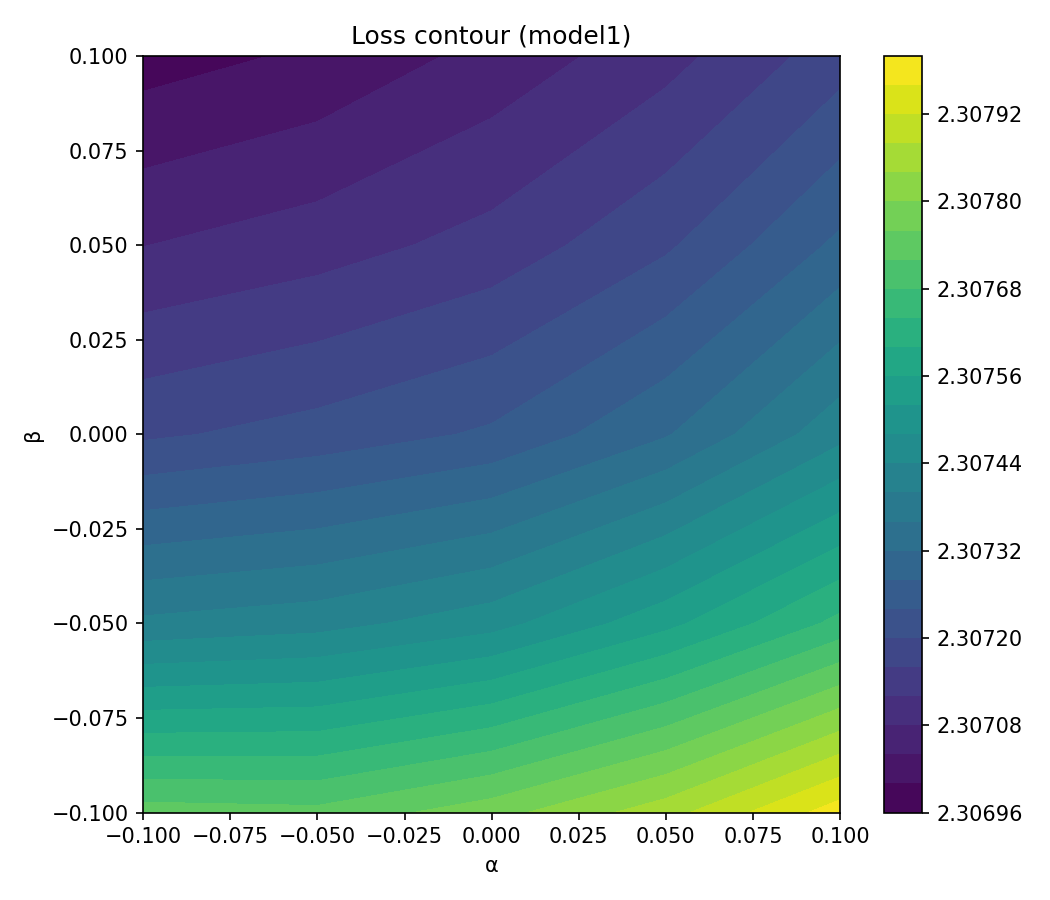
\includegraphics[width=0.85\textwidth]{figures/surface_contour_model1_r0.1.png}
    \caption{Контур исходной поверхности потерь при $r=0.1$.}
    \label{fig:surface_contour}
\end{figure}

\begin{figure}[H]
    \centering
    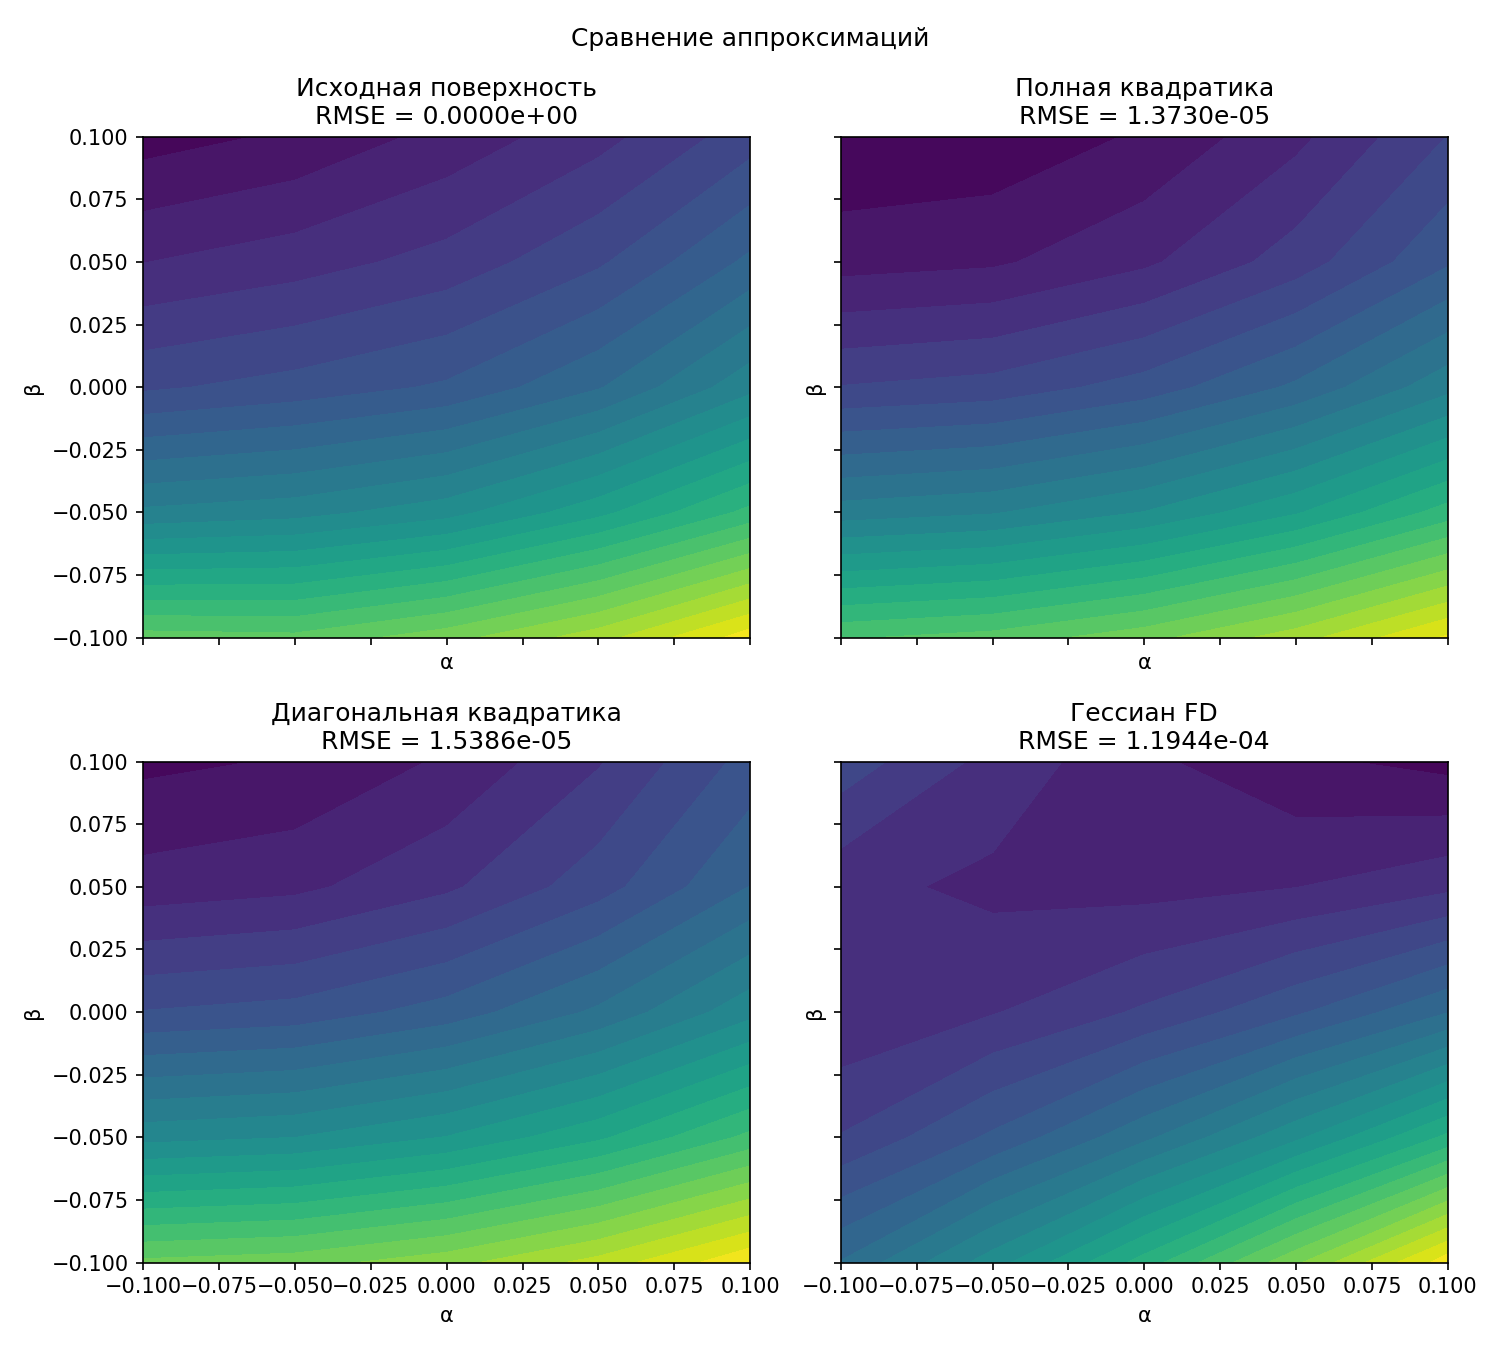
\includegraphics[width=0.85\textwidth]{figures/comparison_model1_r0.1.png}
    \caption{Сравнение исходной поверхности и аппроксимаций $q_1,q_2,q_3$.}
    \label{fig:surface_comparison}
\end{figure}

\begin{figure}[H]
    \centering
    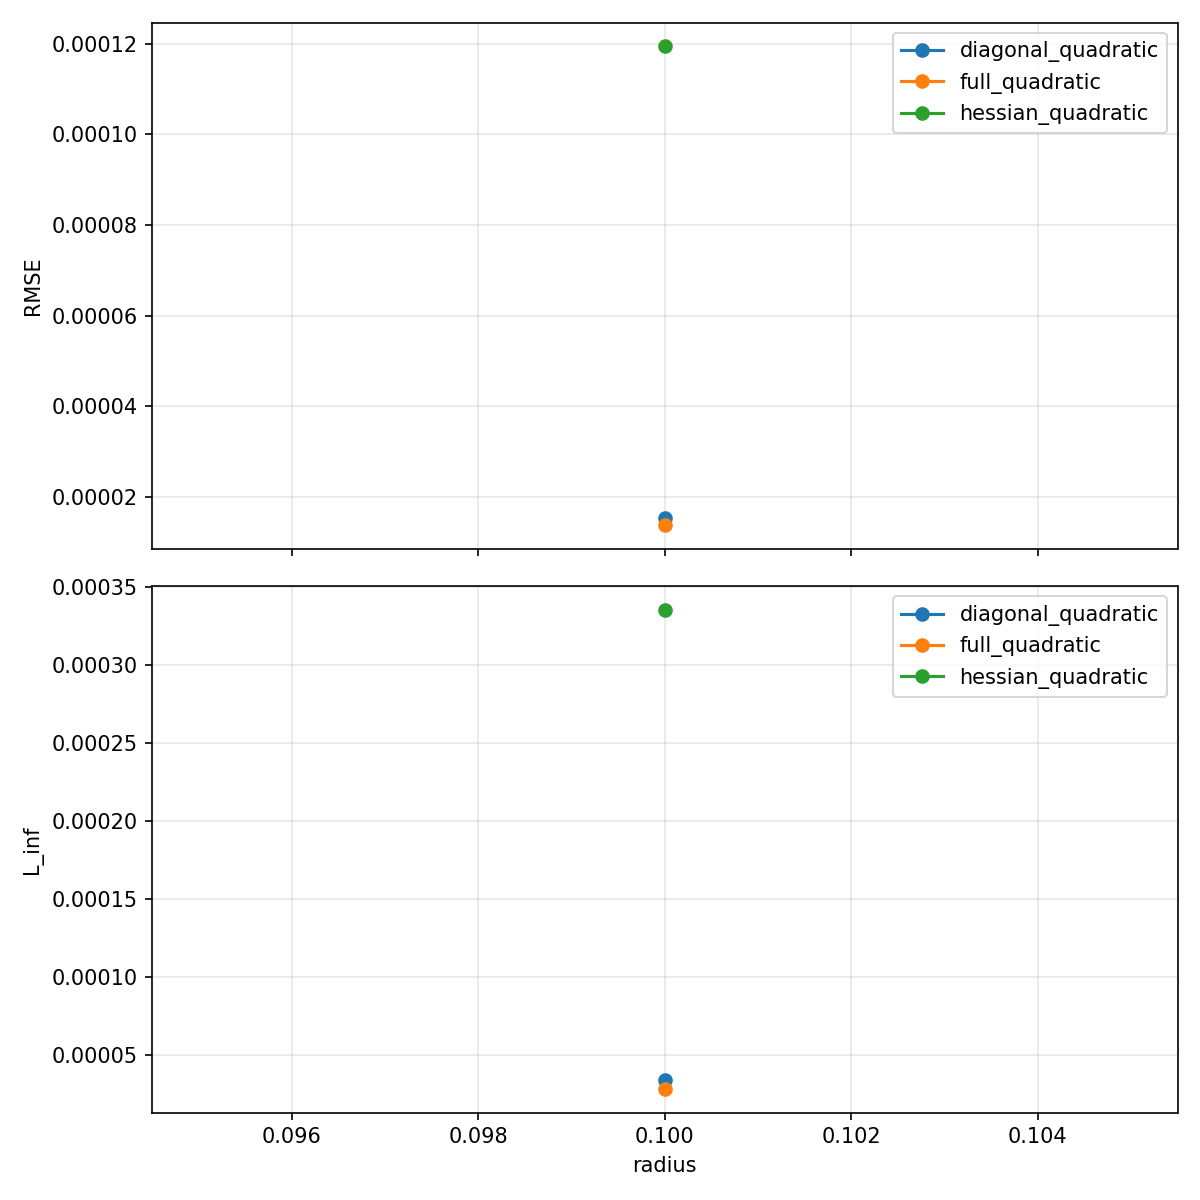
\includegraphics[width=0.85\textwidth]{figures/metrics_vs_radius_model1.png}
    \caption{Зависимость метрик аппроксимации от радиуса.}
    \label{fig:metrics_vs_radius}
\end{figure}
